\documentclass[12pt, a4paper, oneside]{ctexart}
\usepackage{amsmath, amsthm, amssymb, bm, color, graphicx, geometry, mathrsfs,extarrows, braket, booktabs, array, wrapfig, enumitem, subfigure, bbm}
\usepackage[colorlinks,linkcolor=red,anchorcolor=blue,citecolor=blue,urlcolor=blue,menucolor=black]{hyperref}
%%%% 设置中文字体 %%%%
% fc-list -f "%{family}\n" :lang=zh >d:zhfont.txt 命令查看已有字体
\setCJKmainfont[
    BoldFont=方正黑体_GBK,  % 黑体
    ItalicFont=方正楷体_GBK,  % 楷体
    BoldItalicFont=方正粗楷简体,  % 粗楷体
    Mapping = fullwidth-stop  % 将中文句号“.”全部转化为英文句号“.”,
]{方正书宋简体}  % !!! 注意在Windows中运行请改为“方正书宋简体.ttf” !!!
%%%% 设置英文字体 %%%%
\setmainfont{Times New Roman}
\setsansfont{Calibri}
\setmonofont{Fira Code}

%%%% 设置代码块 %%%%
% 在vscode中使用minted需要先配置python解释器, Ctrl+Shift+P, 输入Python: Select Interpreter选择安装了Pygments的Python版本. 再在setting.json中xelatex和pdflatex的参数中加入 "--shell-escape", 即可
% TeXworks中配置方法参考: https://blog.csdn.net/RobertChenGuangzhi/article/details/108140093
\usepackage{minted}
\renewcommand{\theFancyVerbLine}{
    \sffamily\textcolor[rgb]{0.5,0.5,0.5}{\scriptsize\arabic{FancyVerbLine}}} % 修改代码前序号大小
% 加入不同语言的代码块
\newmintinline{cpp}{fontsize=\small, linenos, breaklines, frame=lines}
\newminted{cpp}{fontsize=\small, baselinestretch=1, linenos, breaklines, frame=lines}
\newmintedfile{cpp}{fontsize=\small, baselinestretch=1, linenos, breaklines, frame=lines}
\newminted{r}{fontsize=\fontsize{10pt}{13pt}\selectfont, baselinestretch=1, linenos, breaklines, frame=lines}
\newmintedfile{r}{fontsize=\small, baselinestretch=1, linenos, breaklines, frame=lines}
\newmintinline{matlab}{fontsize=\small, linenos, breaklines, frame=lines}
\newminted{matlab}{fontsize=\small, baselinestretch=1, mathescape, linenos, breaklines, frame=lines}
\newmintedfile{matlab}{fontsize=\small, baselinestretch=1, linenos, breaklines, frame=lines}
\newmintinline{python}{fontsize=\small, linenos, breaklines, frame=lines, python3}  % 使用\pythoninline{代码}
\newminted{python}{fontsize=\small, baselinestretch=1, linenos, breaklines, frame=lines, python3}  % 使用\begin{pythoncode}代码\end{pythoncode}
\newmintedfile{python}{fontsize=\small, baselinestretch=1, linenos, breaklines, frame=lines, python3}  % 使用\pythonfile{代码地址}

%%%% 设置行间距与页边距 %%%%
\linespread{1.4}
%\geometry{left=2.54cm,right=2.54cm,top=3.18cm,bottom=3.18cm}
\geometry{left=1.84cm,right=1.84cm,top=2.18cm,bottom=2.18cm}

%%%% 图片相对路径 %%%%
\graphicspath{{figures/}} % 当前目录下的figures文件夹, {../figures/}则是父目录的figures文件夹
\setlength{\abovecaptionskip}{-0.2cm}  % 缩紧图片标题与图片之间的距离
\setlength{\belowcaptionskip}{0pt} 

%%%% 缩小item,enumerate,description两行间间距 %%%%
\setenumerate[1]{itemsep=0pt,partopsep=0pt,parsep=\parskip,topsep=5pt}
\setitemize[1]{itemsep=0pt,partopsep=0pt,parsep=\parskip,topsep=5pt}
\setdescription{itemsep=0pt,partopsep=0pt,parsep=\parskip,topsep=5pt}

%%%% 自定义公式 %%%%
\everymath{\displaystyle} % 默认全部行间公式
\DeclareMathOperator*\uplim{\overline{lim}} % 定义上极限 \uplim_{}
\DeclareMathOperator*\lowlim{\underline{lim}} % 定义下极限 \lowlim_{}
\DeclareMathOperator*{\argmax}{arg\,max}  % 定义取最大值的参数 \argmax_{}
\DeclareMathOperator*{\argmin}{arg\,min}  % 定义取最小值的参数 \argmin_{}
\let\leq=\leqslant % 将全部leq变为leqslant
\let\geq=\geqslant % geq同理
\DeclareRobustCommand{\rchi}{{\mathpalette\irchi\relax}}
\newcommand{\irchi}[2]{\raisebox{\depth}{$#1\chi$}} % 使用\rchi将\chi居中

%%%% 自定义环境配置 %%%%
\newcounter{problem}  % 问题序号计数器
\newenvironment{problem}[1][]{\stepcounter{problem}\par\noindent\textbf{题目\arabic{problem}. #1}}{\smallskip\par}
\newenvironment{solution}[1][]{\par\noindent\textbf{#1解答. }}{\smallskip\par}  % 可带一个参数表示题号\begin{solution}{题号}
\newenvironment{note}{\par\noindent\textbf{注记. }}{\smallskip\par}
\newenvironment{remark}{\begin{enumerate}[label=\textbf{注\arabic*.}]}{\end{enumerate}}
\BeforeBeginEnvironment{minted}{\vspace{-0.5cm}}  % 缩小minted环境距上文间距
\AfterEndEnvironment{minted}{\vspace{-0.2cm}}  % 缩小minted环境距下文间距

%%%% 一些宏定义 %%%%
\def\bd{\boldsymbol}        % 加粗(向量) boldsymbol
\def\disp{\displaystyle}    % 使用行间公式 displaystyle(默认)
\def\weekto{\rightharpoonup}% 右半箭头
\def\tsty{\textstyle}       % 使用行内公式 textstyle
\def\sign{\textrm{sign}}    % sign function
\def\cov{\textrm{Cov}}      % 
\def\var{\textrm{Var}}      % 
\def\E{\textrm{E}}          % 
\def\T{\textrm{T}}          % 
\def\1{\bd{1}}
\def\wtd{\widetilde}        % 宽波浪线 widetilde
\def\R{\mathbb{R}}          % Real number
\def\N{\mathbb{N}}          % Natural number
\def\Z{\mathbb{Z}}          % Integer number
\def\Q{\mathbb{Q}}          % Rational number
\def\C{\mathbb{C}}          % Complex number
\def\K{\mathbb{K}}          % Number Field
\def\P{\textrm{P}}          % Possibility
\def\d{\mathrm{d}}          % differential operator
\def\e{\mathrm{e}}          % Euler's number
\def\i{\mathrm{i}}          % imaginary number
\def\re{\mathrm{Re}}        % Real part
\def\im{\mathrm{Im}}        % Imaginary part
\def\res{\mathrm{Res}}      % Residue
\def\ker{\mathrm{Ker}}      % Kernel
\def\vspan{\mathrm{vspan}}  % Span  \span与latex内核代码冲突改为\vspan
\def\L{\mathcal{L}}         % Loss function
\def\O{\mathcal{O}}         % big O notation
\def\wdh{\widehat}          % 宽帽子 widehat
\def\ol{\overline}          % 上横线 overline
\def\ul{\underline}         % 下横线 underline
\def\add{\vspace{1ex}}      % 增加行间距
\def\del{\vspace{-1.5ex}}   % 减少行间距

%%%% 定理类环境的定义 %%%%
\newtheorem{theorem}{定理}

%%%% 基本信息 %%%%
\newcommand{\RQ}{\today} % 日期
\newcommand{\km}{数据分析} % 科目
\newcommand{\bj}{强基数学002} % 班级
\newcommand{\xm}{吴天阳} % 姓名
\newcommand{\xh}{2204210460} % 学号

\begin{document}

%\pagestyle{empty}
\pagestyle{plain}
\vspace*{-15ex}
\centerline{\begin{tabular}{*5{c}}
    \parbox[t]{0.25\linewidth}{\begin{center}\textbf{日期}\\ \large \textcolor{blue}{\RQ}\end{center}} 
    & \parbox[t]{0.2\linewidth}{\begin{center}\textbf{科目}\\ \large \textcolor{blue}{\km}\end{center}}
    & \parbox[t]{0.2\linewidth}{\begin{center}\textbf{班级}\\ \large \textcolor{blue}{\bj}\end{center}}
    & \parbox[t]{0.1\linewidth}{\begin{center}\textbf{姓名}\\ \large \textcolor{blue}{\xm}\end{center}}
    & \parbox[t]{0.15\linewidth}{\begin{center}\textbf{学号}\\ \large \textcolor{blue}{\xh}\end{center}} \\ \hline
\end{tabular}}
\begin{center}
    \zihao{3}\textbf{第三次作业}
\end{center}\vspace{-0.2cm}
\begin{problem}
    对于过原点的简单线性回归模型
    \begin{equation*}
        y_i = \beta x_i + \varepsilon_i,\quad i=1,2,\cdots,n,
    \end{equation*}
    设$\varepsilon_i(i=1,2,\cdots,n)$相互独立且服从$N(0,\sigma^2)$分布。

    \begin{enumerate}[label={(\arabic*)}]
        \item 求$\beta$的最小二乘估计,它是否是$\beta$的无偏估计?
        \item 求出误差方差$\sigma^2$的一个无偏估计
        \item 写出回归关系显著性检验的统计量及其零分布,相应的方差分析表,它和具有常数项的简单线性回归模型的
        相应结果有何区别?
        \item 给出检验假设$H_0:\beta = 0$的$t$统计量及其零分布,它和(3)中的假设检验有何关系?
        \item 对于自变量的新的观测值$x_0$,给出相应的因变量取值$y_0$的预测值及其置信度为$1-\alpha$的置信区间。
    \end{enumerate}
\end{problem}
\begin{solution}
    (1)  $\beta$的最小二乘估计,即最小化残差平方和$S(\beta) = \sum_{i=1}^n (y_i-\beta x_i)^2$。
    对$\beta$求导并令其等于0,可得
    \begin{align*}
        \frac{\partial}{\partial \beta}\sum_{i=1}^n (y_i-\beta x_i)^2 = -2\sum_{i=1}^n x_i(y_i-\beta x_i)
        = -2\sum_{i=1}^n x_i y_i + 2\beta\sum_{i=1}^n x_i^2 = 0.
    \end{align*}
    解得$\hat{\beta}=\frac{\sum_{i=1}^n x_i y_i}{\sum_{i=1}^n x_i^2}$。\add

    下证$\hat{\beta}$为$\beta$的无偏估计。由于
    $\E(Y)=\E(\beta X+\varepsilon)=\beta X$,
    所以
    \begin{align*}
        \E(\hat{\beta})
        = \E\left(\frac{\sum_{i=1}^n x_i y_i}{\sum_{i=1}^n x_i^2}\right) 
        = \frac{\sum_{i=1}^n x_i \E(y_i)}{\sum_{i=1}^n x_i^2} 
        = \frac{\sum_{i=1}^n x_i (\beta x_i)}{\sum_{i=1}^n x_i^2} 
        = \beta.
    \end{align*} 故,$\hat{\beta}$是$\beta$的无偏估计。

    (2) 
    由于残差平方和$\text{SSE}=\hat{\bd{\varepsilon}}^{\T}\hat{\bd{\varepsilon}}=\sum_{i=1}^n (y_i-\hat{\beta}x_i)^2$满足$\E(\text{SSE}) = \sigma^2(n-1)$,
    从而$\sigma^2$的一个无偏估计为$\hat{\sigma}^2 = \frac{\text{SSE}}{n-1} = \frac{1}{n-1}\sum_{i=1}^n (y_i-\hat{\beta}x_i)^2$.

    (3) 令原假设为$H_0:\beta=0$,备择假设为$H_1:\beta\neq 0$,则显著性检验统计量取为
    \begin{equation*}
        F = \frac{\text{MSR}}{\text{MSE}} = \frac{\text{SSR}}{\text{SSE}/(n-1)} = \frac{\sum_{i=1}^n(\hat{y}_i - \bar{y})^2}{\sum_{i=1}^n(y_i-\hat{\beta}x_i)^2/(n-1)}
    \end{equation*}
    其中$\text{SSR}$可进一步简化,
    \begin{align*}
        \text{SSR} =&\ \sum_{i=1}^n(\hat{y}_i-\bar{y})^2 = \sum_{i=1}^n\left(\hat{\beta} x_i - \frac{1}{n}\sum_{i=1}^n\hat{\beta} x_i\right)^2 = \sum_{i=1}^n\hat{\beta}^2x_i^2 - 2\sum_{i=1}^n\hat{\beta}^2x_i\bar{y} + n\bar{y}^2\\
        =&\ \sum_{i=1}^n\hat{\beta}^2x_i^2 - \frac{2\beta^2}{n}\sum_{i,j}x_ix_j + \frac{\beta^2}{n}\left(\sum_{i=1}^nx_i\right)^2 = \frac{n-1}{n}\hat{\beta}^2\sum_{i=1}^nx_i^2
    \end{align*}
    于是检验统计量\add $F = \frac{(n-1)^2}{n}\frac{\hat{\beta}^2\sum_{i=1}^nx_i^2}{\sum_{i=1}^n(y_i-\hat{\beta}^2x_i)^2}$,零分布为$F(1,n-1)$;
    假设$F$的观测值为$F_0$,当$p_0 = \P_{H_0}(F(1,n-1)> F_0) < \alpha$时,拒绝原假设,认为自变量$x$对因变量$y$有显著性关系。

    方差分析表如下:
    \renewcommand\arraystretch{0.8} % 设置表格高度为原来的0.8倍
    \begin{table}[!htbp] % table标准
        \centering % 表格居中
        \begin{tabular}{p{3cm}<{\centering}p{2cm}<{\centering}p{2cm}<{\centering}p{4cm}<{\centering}p{3cm}<{\centering}} % 设置表格宽度
        %\begin{tabular}{cccc}
            \toprule
            方差来源 & 自由度 &平方和 &  均方和 & F值 \\
            \midrule
            回归(R) & 1 & SSR & MSR=SSR & F=MSR/MSE \\
            残差(E) & n-1 & SSE & MSE=SSE/(n-1) & \\
            总和(T) & n & SST & &\\
            \bottomrule
        \end{tabular}
    \end{table}

    和具有常数项的简单线性回归相比,回归平方和的自由度由于少了常数项,所以自由度增加$1$,所以总的自由度为$n$,而带有常数项的总自由度为$n-1$.\add

    (4) 假设检验$H_0 : \beta = 0$的$t$统计量为$t = \frac{\hat{\beta}}{s(\hat{\beta})} = \frac{\hat{\beta}}{\sqrt{\text{MSE} / (\sum_{i=1}^nx_i^2)}}$,
    假设原假设成立,则$t\sim t(n-1)$,不难发现,当$n\to\infty$时,(3)小问中的统计量近似为$F = \frac{\hat{\beta}^2\sum_{i=1}^nx_i^2}{\text{MSE}} = t^2$\add,
    于是假设当$t,F$的观测值为$t_0,F_0$,则$t_0^2 = F_0$,并且
    \begin{equation*}
        \P(t > |t_0|) = \P(t^2 > t_0^2) = \P(F > F_0)
    \end{equation*}
    所以二者的拒绝域相同,故两个检验统计量等价。

    (5) 由简单线性回归模型可知,新的观测值$x_0$对应的预测值为$\hat{y}_0 = \hat{\beta}x_0$,且有
    \begin{equation*}
        \frac{\hat{y}_0 - y_0}{\sqrt{\text{MSE} (1 + \frac{x_0^2}{\sum_{i=1}^nx_i^2})}}\sim t(n-1)   
    \end{equation*}
    于是对于假设$H_0:\hat{y}_0 = y_0$的$1-\alpha$置信区间为
    \begin{equation*}
        \hat{\beta}x_0 \pm t_{1-\frac{\alpha}{2}}(n-1)\sqrt{\text{MSE}(1 + \frac{x_0^2}{\sum_{i=1}^nx_i^2})}
    \end{equation*}
\end{solution}

\begin{problem}
    考察下列回归模型
    \begin{equation*}
        y_i = \beta_0+\beta_1x_{i1}+\beta_2x_{i2}+\beta_3x_{i1}x_{i2}+\beta_4\sqrt{x_{i3}}+\varepsilon_i,\quad i=1,2,\cdots,n,
    \end{equation*}
    并假设误差项独立同分布于$N(0,\sigma^2)$。在下列情况下,写出简约模型、相应的检验检验统计量及其零分布:
    \begin{enumerate}[label={(\arabic*)}]
        \item $\beta_3=\beta_4=0$;
        \item $\beta_1=\beta_2$;
        \item $\beta_4 = 1$.
    \end{enumerate}
\end{problem}
\begin{solution}
    令$Z_1= X_1X_2, Z_2 = \sqrt{X_3}$,则全模型为$Y = \beta_0 + \beta_1X_1 + \beta_2X_2 + \beta_3Z_1 + \beta_4Z_2 + \varepsilon$,全模型残差平方和自由度为$f_F = n-5$。

    (1) 约简模型为$Y = \beta_0+\beta_1X_1+\beta_2X_2+\varepsilon_i$,残差平方和自由度为$f_R = n-3$,
    于是检验统计量及对应的零分布为
    \begin{equation*}
        F = \frac{[\text{SSE}(R) - \text{SSE}(F)]/(f_R-f_F)}{\text{SSE}(F)/f_F} = \frac{[\text{SSE}(R)-\text{SSE}(F)]/2}{\text{SSE}(F)/(n-5)}\sim F(2,n-5).
    \end{equation*}

    (2) 令$Z_3 = X_1+X_2$,则约简模型为$Y = \beta_0 + \beta_1(X_1+X_2) + \beta_3Z_1 + \beta_4Z_2+\varepsilon = \beta_0 + \beta_1Z_3 + \beta_3Z_1 + \beta_4Z_2 + \varepsilon$,
    $f_R = n-4$,于是检验统计量及对应的零分布为
    \begin{equation*}
        F = \frac{\text{SSE}(R) - \text{SSE}(F)}{\text{SSE}(F) / (n-5)} \sim F(1,n-5)
    \end{equation*}

    (3) 约简模型为$Y = \beta_0 + \beta_1X_1+\beta_2X_2+\beta_3Z_1 + Z_2 + \varepsilon$,将其改写为$\wtd{Y} = Y - Z_2 = \beta_0 + \beta_1X_1+\beta_2X_2+\beta_3Z_1 + \varepsilon$,
    此时$\wtd{Y}$的观测值为$\tilde{y}_i = y_i-z_{i2} = y_i - \sqrt{x_{i3}}$,且$f_R = n-4$,于是检验统计量及对应的零分布为
    \begin{equation*}
        F = \frac{\text{SSE}_{\wtd{Y}}(R) - \text{SSE}(F)}{\text{SSE}(F) / (n-5)} \sim F(1,n-5)
    \end{equation*}
\end{solution}
\vspace{-0.5cm}
\begin{problem}
    某公司为了分析某化妆品的月销量$Y$与使用人数$X_1$,及人均月收入$X_2$之间的关系,得到$15$组观测值,如书上表2.16所示。假设$Y$与$X_1,X_2$之间满足线性回归关系
    \begin{equation*}
        y_i = \beta_0+\beta_1x_{i1}+\beta_2x_{i2}+\varepsilon_i,\quad i=1,2,\cdots,15,
    \end{equation*}
    其中$\varepsilon_i(i=1,2,\cdots,15)$独立同分布于$N(0,\sigma^2)$。

    (1) 求回归系数$\beta_0,\beta_1,\beta_2$的最小二乘估计和误差方差$\sigma^2$的估计,写出回归方程并对回归系数作解释。

    (2) 给出方差分析表,解释对线性回归关系显著性检验的结果,求复相关系数的平方$R^2$的值,并解释其意义。

    (3) 分别求$\beta_1$和$\beta_2$的置信度为$95\%$的置信区间。

    (4) 对$\alpha = 0.05$,分别检验人数$X_1$及收入$X_2$对销量$Y$的影响是否显著,利用与回归系数有关的一般假设检验方法检验$X_1$和$X_2$的交互作用(即$X_1X_2$)对$Y$的影响是否显著。

    (5) 该公司欲在一个适宜使用该化妆品的人数$x_{01} = 220$,人均月收入$x_{02} = 2500$的新城市中销售该化妆品,求其销售量的预测值及其置信度为$95\%$的置信区间。

    (6) 求$Y$的拟合值、残差及学生化残差,根据学生化残差正态性的频率检验及正态QQ图检验说明模型误差项的正态性假定是否合理,有序学生化残差与相应标准正态分布的分位数的相关系数是多少?作出各种残差图,分析模型有关假定的合理性。
\end{problem}
\begin{solution}
    (1) 使用R语言中的\texttt{lm()}函数拟合线性回归模型:
    \begin{rcode}
> data <- read.table(file = "exercise_2.4.txt")
> colnames(data) <- c("Y", "X1", "X2")
> fit <- lm(Y ~ X1 + X2, data = data)
> coef(fit)  # 输出系数
(Intercept)          X1          X2 
3.452612790 4.960049761 0.009199081
> summary(fit)$sigma  # 输出方差估计
[1] 2.177222
    \end{rcode}
    从输出结果可知,$\beta_0,\beta_1,\beta_2$最小二乘估计分别为$3.45,4.96,0.0092$,
    误差方差$\sigma^2$的估计为$\hat{\sigma}^2 = 2.177$,回归方程为
    $\hat{y} = 3.45 + 4.96x_1 + 0.0092x_2+\varepsilon$,从回归系数可以看出,
    由于没有对收入进行归一化,所以系数较小。

    (2) 
    \begin{rcode}
> anova(fit)  # 输出方差分析表
Analysis of Variance Table

Response: Y
          Df Sum Sq Mean Sq   F value    Pr(>F)    
X1         1  53417   53417 11268.644 < 2.2e-16 ***
X2         1    428     428    90.289 6.201e-07 ***
Residuals 12     57       5                        
---
Signif. codes:  0 ‘***’ 0.001 ‘**’ 0.01 ‘*’ 0.05 ‘.’ 0.1 ‘ ’ 1
> summary(fit)$fstatistic  # 输出显著性检验统计量F,分子对应的自由度,分母对应的自由度
   value    numdf    dendf 
5679.466    2.000   12.000 
# 使用pf()函数计算F分布的累计分布函数,求出检验p值大小
> pf(summary(fit)$fstatistic[1], summary(fit)$fstatistic[2], summary(fit)$fstatistic[3], lower.tail = FALSE)
       value 
1.381373e-18 
> summary(fit)$r.squared  # 输出复相关系数R2
[1] 0.9989447
    \end{rcode}
    从上述输出结果可知,检验$p$值为$1.38\times 10^{-18}$,远小于$0.05$,说明检验$Y$与$X_1,X_2$之间有显著性关系。
    复相关系数$R^2 = 0.9989447$非常接近$1$,也说明$Y$与$X_1,X_2$的线性关系显著。

(3) 
\begin{rcode}
> confint(fit, level = 0.95)  # 求95%的置信度区间
                   2.5 %     97.5 %
(Intercept) -1.843319690 8.74854527
X1           4.828134820 5.09196470
X2           0.007089742 0.01130842
\end{rcode}
通过上述输出结果可知,$95\%$的置信区间分别为$\beta_1:[4.828,5.092],\beta_2:[0.0071,0.0113]$。

(4)
\begin{rcode}
> summary(fit)$coefficients  # 输出每个系数的显著性检验p值
               Estimate   Std. Error   t value     Pr(>|t|)
(Intercept) 3.452612790 2.4306504934  1.420448 1.809353e-01
X1          4.960049761 0.0605444118 81.924155 7.296818e-18
X2          0.009199081 0.0009681139  9.502065 6.201181e-07
\end{rcode}
从上述输出结果可知,由于$7.3\times10^{-18},6.2\times10^{-7}$均小于显著性水平$0.05$,所以拒绝原假设,
即认为$X_1,X_2$均对$Y$的影响显著。

下面在原模型的基础上增加一个交互项$X_1X_2$,然后再使用上述方式进行检验:
\begin{rcode}
> fit2 <- lm(Y ~ X1 * X2, data = data)
> summary(fit2)$coefficients
                Estimate   Std. Error    t value     Pr(>|t|)
(Intercept) 4.9011280216 8.538689e+00  0.5739907 5.775222e-01
X1          4.9110125459 2.831608e-01 17.3435481 2.450885e-09
X2          0.0086738979 3.123930e-03  2.7765976 1.801319e-02
X1:X2       0.0000169767 9.556168e-05  0.1776517 8.622257e-01
\end{rcode}
从上述输出结果可知,由于$0.862 > 0.05$,所以接受原假设,即$X_1X_2$对$Y$的影响并不显著。

(5)
\begin{rcode}
> newdata <- data.frame(X1 = 220, X2 = 2500)  # 创建新数据
# 对新数据进行预测,并求出置信度为95%的置信区间
> predict(fit, newdata = newdata, interval = "confidence", level = 0.95)
       fit      lwr      upr
1 1117.661 1091.234 1144.088
\end{rcode}
从上输出结果可知,销售量的预测值为$\hat{y}_0 = 1118$,$95\%$的置信区间为$[1091.234,1144.088]$.

(6) 
\begin{rcode}
> fitted(fit)  # 计算每个样本对应的拟合值
    1         2         3         4         5         6         7         8 
161.89572 122.66732 224.42938 131.24062  67.69928 169.68486  79.73194 189.67200 
    9        10        11        12        13        14        15 
119.83202  53.29052 253.71506 228.69079 144.97934 100.53307 210.93806
> resid(fit)  # 计算每个样本对应的残差
         1          2          3          4          5          6          7 
 0.1042756 -2.6673176 -1.4293843 -0.2406244 -0.6992835 -0.6848553  1.2680643 
         8          9         10         11         12         13         14 
 2.3279970 -3.8320189  1.7094765 -1.7150576  3.3092051 -0.9793423  2.4669251 
        15 
 1.0619404 
> rstudent(fit)  # 计算每个样本对应的学生化残差
 1           2           3           4           5           6 
0.04973473 -1.36670170 -0.71265041 -0.11000544 -0.34443368 -0.33365032 
 7           8           9          10          11          12 
0.65018013  1.25776219 -2.21655274  0.91079624 -0.92397237  2.16085046 
13          14          15 
-0.45379850  1.27498091  0.55945704 

# 可以使用Shapiro-Wilk检验对学生化残差正态性的频率进行检验
> shapiro.test(rstudent(fit))

    Shapiro-Wilk normality test

data:  rstudent(fit)
W = 0.98919, p-value = 0.999

# 学生化残差和相应标准正态分布的分位数的相关系数
> cor(rstudent(fit), qnorm(ppoints(length(rstudent(fit)))))
[1] 0.3719642

# 输出残差图和QQ图
> plot(fit)
\end{rcode}
上述输出结果给出了$Y$的拟合值、残差及学生化残差,学生化残差正态性的频率检验给出的检验$p$值为$0.999$说明,无法拒绝原假设,
即学生化残差符合正态分布;学生化残差和相应标准正态分布的分位数的相关系数为$0.37$;残差图和QQ图如图1所示,通过QQ图可以看出
所有样本基本在同一条直线上,也能说明模型误差项的正态性假设合理;残差图中可以看出,残差分布在$0$附近,第$2,9,12$个样本为离群值,
应检查这三个观测值是否为异常值。
%%%% 两组图并排放(可溢出一些) %%%%
\begin{figure}[H]
    \hspace{-2.2cm}
    \subfigure  % 子图的标题
    {
        % 如果一行放三个图改成0.3\linewidth即可
        \begin{minipage}[b]{.62\linewidth}
            \centering
            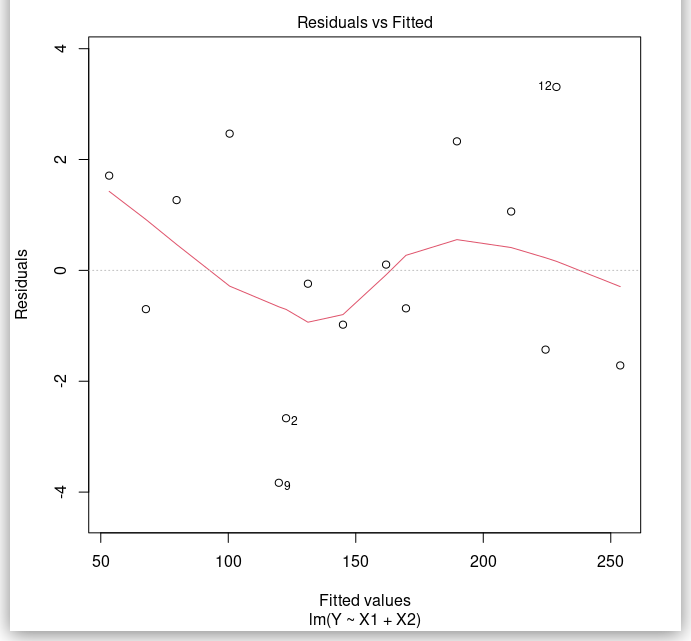
\includegraphics[scale=0.4]{./figures/2.4残差图.png}
        \end{minipage}
    }
    \subfigure
    {
        \begin{minipage}[b]{.2\linewidth}
            \centering
            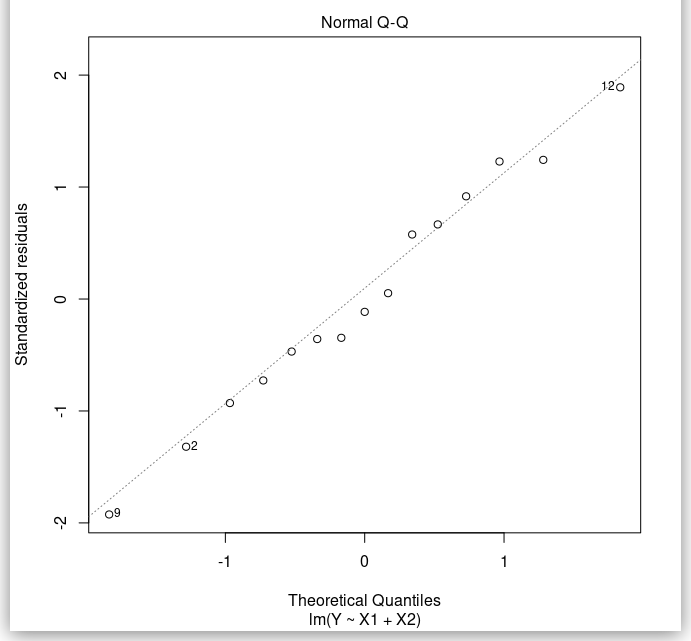
\includegraphics[scale=0.4]{./figures/2.4QQ图.png}
        \end{minipage}
    }
    \caption{残差图和QQ图}
\end{figure}
\end{solution}
\begin{problem}
    在林业工程中,需要研究树干体积$Y$与离地面一定高度的树干直径$X_1$和树干高度$X_2$之间的关系,书上表2.18给出了$31$课树的相关信息。

    (1) 首先拟合线性回归模型$Y =\beta_0+\beta_1X_1+\beta_2X_2+\varepsilon$,通过残差分析考察模型的合理性,是否需要对数据作变换?

    (2) 对因变量$Y$做Box-Cox变换,确定变换参数$\lambda$的值。对变换后的因变量重新拟合与$X_1,X_2$的线性回归模型并作残差分析,Box-Cox变换的效果如何?
\end{problem}
\begin{solution}
    (1) 
\begin{rcode}
> data <- read.table(file = "exercise2_6.txt")
> colnames(data) <- c("X1", "X2", "Y")
> fit <- lm(Y ~ X1 + X2, data = data)
> coef(fit)  # 输出系数
(Intercept)          X1          X2 
-57.9876589   4.7081605   0.3392512 
> plot(fit)  # 输出残差图
\end{rcode}

\begin{wrapfigure}[13]{r}{.5\linewidth} % 文字环绕行数为13行, 图片靠右 (l为靠左), 图片占0.5的行宽
    \vspace{-0.5cm}
    \centering
    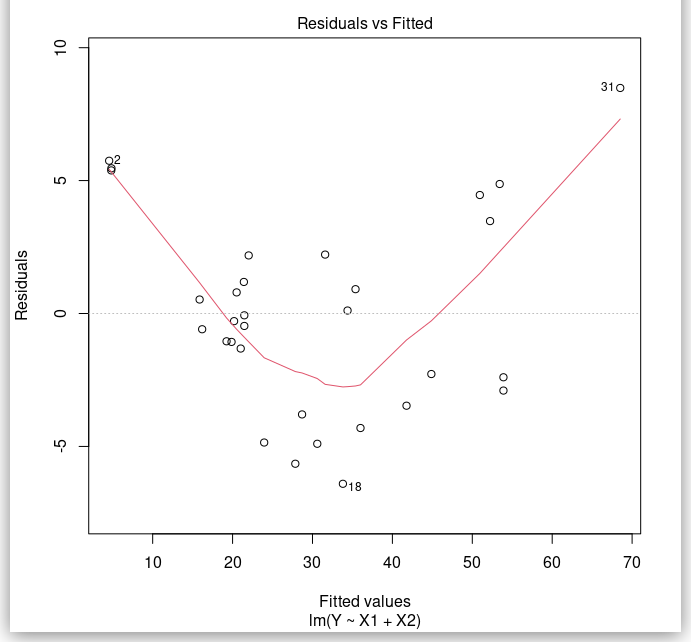
\includegraphics[scale=0.3]{./figures/2.6残差图.png}
    \caption{残差图}
\end{wrapfigure}
通过上述代码可知通过最小二乘拟合得到的线性回归模型为
\begin{equation*}
    y = -57.988 + 4.708x_1 + 0.339x_2 + \varepsilon
\end{equation*}
残差图如右图2所示,从该图可以得知,回归函数可能是非线性的,需要引入某个自变量的二次项或多个自变量的交叉乘积项。

\ 

\ 
% 这里一定要空一行

(2) \begin{rcode}
> library(MASS)  # 导入boxcox依赖包
> bc_result <- boxcox(fit)  # 进行boxcox变换,绘制出对数似然图像
> lambda <- bc_result$x[which.max(bc_result$y)]  # 取对数似然最大处的lambda
> lambda  # 输出参数lambda
[1] 0.3030303

# 对Y做Box-Cox变换
> if (lambda == 0) {
  Y_trans <- log(data$Y)
} else {
  Y_trans <- (data$Y^lambda - 1) / lambda
}
> data$Y_trans <- Y_trans  # 将变换后的数据加入到data中
> fit_trans <- lm(Y_trans ~ X1 + X2, data = data)  # 重新拟合
> plot(fit_trans)  # 绘制Box-Cox变换后的残差图
\end{rcode}
%%%% 两组图并排放(可溢出一些) %%%%
\begin{figure}[htbp]
    \hspace{-2.2cm}
    \subfigure  % 子图的标题
    {
        % 如果一行放三个图改成0.3\linewidth即可
        \begin{minipage}[b]{.62\linewidth}
            \centering
            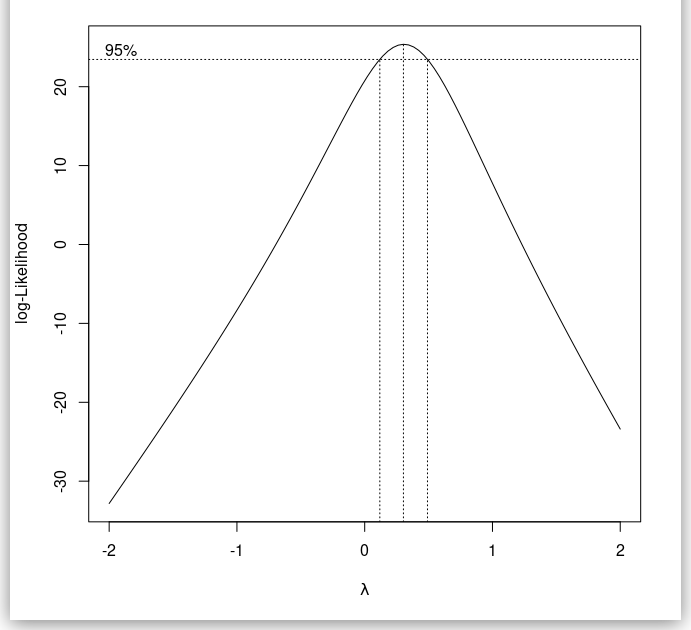
\includegraphics[scale=0.4]{./figures/2.6最大似然确定Box-Cox中参数Lambda.png}
        \end{minipage}
    }
    \subfigure
    {
        \begin{minipage}[b]{.2\linewidth}
            \centering
            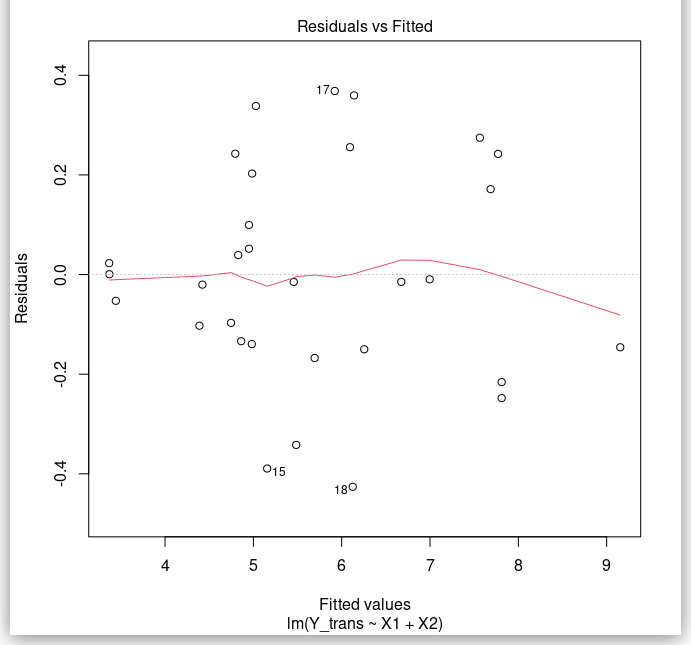
\includegraphics[scale=0.4]{./figures/2.6Box-Cox变换后的残差图.png}
        \end{minipage}
    }
    \caption{对数似然图像和Box-Cox变换后的残差图}
\end{figure}
通过执行代码,可得到上图3中$Y^{(\lambda)}$的对数似然图像\add,选取最大处的值$\lambda = 0.303$;再对$Y$做Box-Cox变换,
得到$Y^{(\lambda)} = \frac{Y^{\lambda}-1}{\lambda}$,\add 最后重新对$X_1,X_2$进行拟合,得到图3右图所示的残差图,
可以看出残差值大致分布在水平带状区域,且不呈现任何明显趋势,可以认为$\varepsilon\sim N(0,\sigma^2)$假设合理,
故Box-Cox变换效果较好。
\end{solution}
\begin{problem}
    在上题中,由于树干可近似地看作圆柱或圆台,于是考虑线性回归模型
    \begin{equation*}
        Y=\beta_0+\beta_1X_1^2+\beta_2X_2+\varepsilon
    \end{equation*}
    可能更为合理。利用书上表2.18数据拟合此模型,进行2.6题同样的分析,并与2.6题结果作比较。
\end{problem}
\begin{solution}
    \begin{rcode}
> fit_quad <- lm(Y ~ I(X1^2) + X2, data = data)
> coef(fit_quad)
(Intercept)     I(X1^2)          X2 
-27.5116027   0.1684577   0.3488088

> plot(fit_quad)  # 绘制残差图
    \end{rcode}

\begin{wrapfigure}[8]{r}{.5\linewidth} % 文字环绕行数为13行, 图片靠右 (l为靠左), 图片占0.5的行宽
    \vspace{-0.5cm}
    \centering
    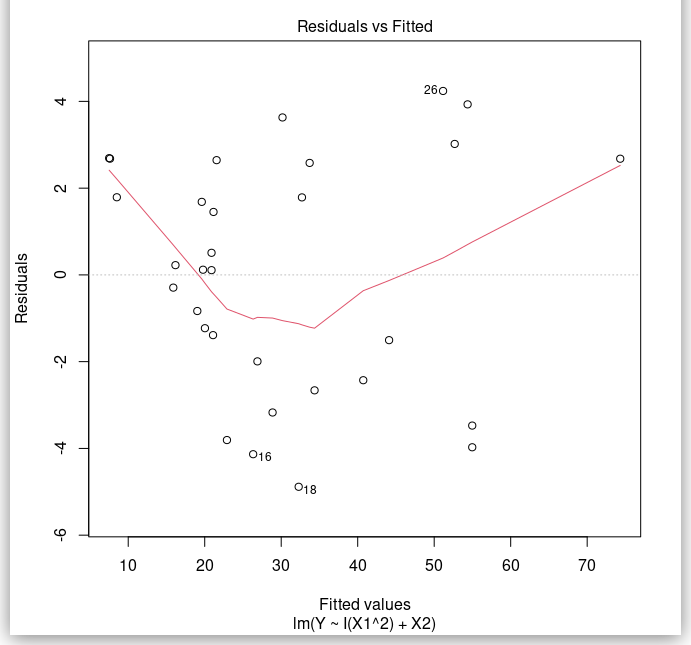
\includegraphics[scale=0.3]{./figures/2.7残差图.png}
    \caption{残差图}
\end{wrapfigure}
    通过上述代码可知拟合得到的线性模型为
    \begin{equation*}
        y = -27.512 + 0.168x_1^2 + 0.349x_2+\varepsilon
    \end{equation*}
    残差图如右图4所示,与上题的图2相比,方差有明显降低,并且残差大致分布在水平带状区域,没有明显的趋势,
    说明将$X_1$修改为$X_1^2$更为合理。
    
    \ 

    \ 

    \ 
\end{solution}

\begin{problem}
    某医院为了解患者对医院的满意程度$Y$和患者的年龄$X_1$,病情的严重程度$X_2$和患者的忧虑程度$X_3$之间的关系,
    随机调查了该医院的$23$位患者,数据如书上表2.19所示。

    (1) 拟合线性模型$Y = \beta_0 + \beta_1X_1+\beta_2X_2+ \beta_3X_3 + \varepsilon$,通过残差分析考察模型
    及有关误差分析正态性假定的合理性;

    (2) 若(1)中模型合理,分别在(i) $R_a^2(p)$、(ii) $C_p$ 和 (iii) $\text{PRESS}_p$ 准则下选择最优回归方程,
    各准则下的选择结果是否一致?

    (3) 对$\alpha_E = \alpha_D = 0.10$,用逐步回归法选择最优回归方程,其结果和$(2)$中的是否一致?

    (4) 对选择的最优回归方程作残差分析,与(1)中的相应结果比较,有何变化?
\end{problem}

\ 
\begin{solution}
    (1)
    \begin{rcode}
> data <- read.table("exercise2_9.txt")
> colnames(data) <- c("X1", "X2", "X3", "Y")
> fit <- lm(Y ~ X1 + X2 + X3, data = data)
> coef(fit)
(Intercept)          X1          X2          X3 
162.8758987  -1.2103182  -0.6659056  -8.6130315 
> plot(fit)
> shapiro.test(fit$residuals)  # 使用Shapiro-Wilk检验对残差正态性进行检验

    Shapiro-Wilk normality test

data:  fit$residuals
W = 0.95393, p-value = 0.3522

    \end{rcode}

\begin{wrapfigure}[11]{r}{.5\linewidth} % 文字环绕行数为13行, 图片靠右 (l为靠左), 图片占0.5的行宽
    \vspace{-0.5cm}
    \centering
    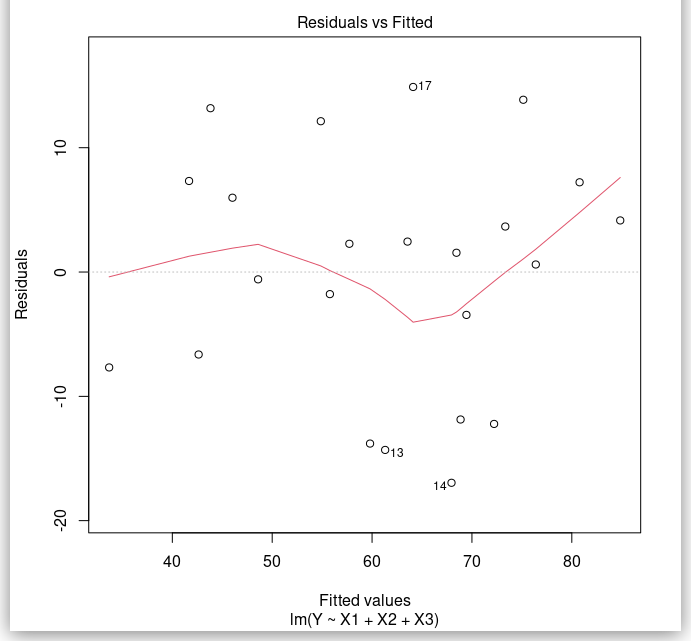
\includegraphics[scale=0.3]{./figures/2.9残差图.png}
    \caption{残差图}
\end{wrapfigure}
    通过上述代码得到拟合结果为
    \begin{equation*}
        y = 162.876  -1.210x_1 -0.666x_2 - 8.613x_3 + \varepsilon
    \end{equation*}
    残差图如右图5所示,从该图可以得知,残差值分布在水平带状区域中,所以模型合理;并且通过Shapiro-Wilk对残差正态性
    进行检验,得到检验p值为$0.3522 > 0.05$,所以可以接受原假设,即残差分布符合正态性假定。

    (2) 用函数\texttt{model\_selection}枚举全部自变量组合,并输出每种组合下的\\$R_a^2,C_p,\text{PRESS}_p$值
    \rfile{./model_selection.R}
    \begin{rcode}
> source("../model_selection.R")
> model_selection(data, "Y", c("X1", "X2", "X3"))
  Predictors      Ra.2       Cp   PRESSp
1         X1 0.5794702 125.6640 3024.209
2         X2 0.3139047 193.3935 4853.280
3         X3 0.3324340 188.6678 4652.835
4     X1, X2 0.6305423 117.3580 2714.105
5     X1, X3 0.6274569 118.1075 2693.434
6     X2, X3 0.3344295 189.2821 4966.428
7 X1, X2, X3 0.6209731 124.2855 3046.291
    \end{rcode}
    通过上述代码执行结果可知,三个参数最优取值均有$X_1$,两个参数的最优取值有$X_2$,一个参数的最优取值有$X_3$,
    并且$X_1,X_2$在两个参数取值下均为最优;
    综合可知,最优参数选择应该为$X_1,X_2$。

    (3) 由于R语言中没有指定$\alpha_E$和$\alpha_D$值的函数,只能使用AIC、BIC准则进行逐步回归
    \begin{rcode}
> full_model <- lm(Y ~ X1 + X2 + X3, data = data)
> step_model <- step(full_model, direction = "both", k = log(nrow(data)))
Start:  AIC=115.38
Y ~ X1 + X2 + X3

       Df Sum of Sq    RSS    AIC
- X3    1     52.41 2064.0 112.83
- X2    1     69.65 2081.2 113.03
<none>              2011.6 115.38
- X1    1   1706.67 3718.3 126.37

Step:  AIC=112.84
Y ~ X1 + X2

       Df Sum of Sq    RSS    AIC
<none>              2064.0 112.83
- X2    1    402.78 2466.8 113.80
+ X3    1     52.41 2011.6 115.38
- X1    1   1960.56 4024.6 125.06
    \end{rcode}
    第一步,包含$X_1,X_2,X_3$三个参数,删除$X_3$参数,AIC值从115.38降至112.83,因此将其删去;第二步,模型只有$X_1,X_2$两个参数,
    由于没有任何操作可以降低AIC值,所以停止逐步回归,得到最优回归方程,包含参数$X_1,X_2$,并且与(2)结果一致。

    (4) 
    \begin{rcode}
> coef(step_model)
(Intercept)          X1          X2 
 166.591330   -1.260458   -1.089318
> plot(step_model)  # 绘制残差图
> shapiro.test(step_model$residuals)  # 使用 Shapiro-Wilk 检验对残差正态性进行检验

    Shapiro-Wilk normality test

data:  step_model$residuals
W = 0.95651, p-value = 0.3967
    \end{rcode}

\begin{wrapfigure}[10]{r}{.5\linewidth} % 文字环绕行数为13行, 图片靠右 (l为靠左), 图片占0.5的行宽
    \vspace{-0.5cm}
    \centering
    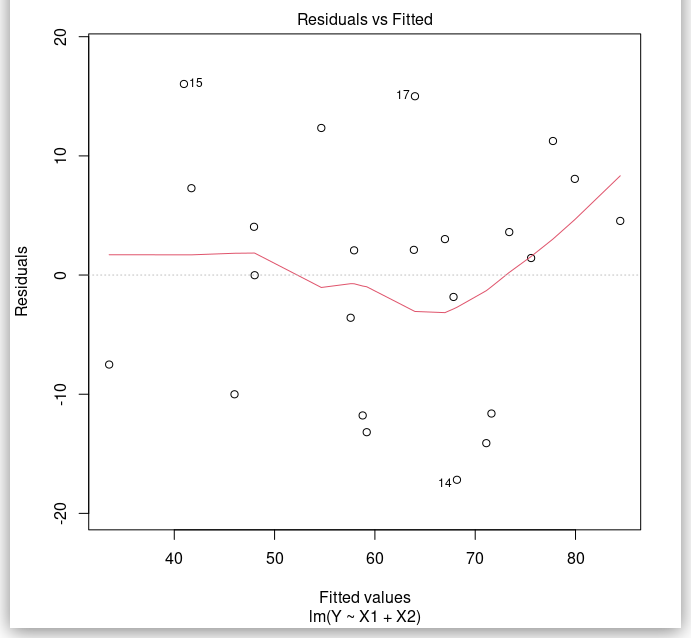
\includegraphics[scale=0.3]{./figures/2.9残差图step.png}
    \caption{残差图}
\end{wrapfigure}
    通过上述代码得到拟合结果为
    \begin{equation*}
        y = 166.591  -1.260x_1 -1.089x_2 + \varepsilon
    \end{equation*}
    残差图如右图6所示,从该图可以得知,残差值分布在水平带状区域中,所以模型合理;并且通过Shapiro-Wilk对残差正态性
    进行检验,得到检验p值为$0.3967$大于(1)中的$0.3522$,所以说明模型拟合效果更好。

    \ 

    \ 

    \ 
\end{solution}
\begin{problem}
    书上表2.20是66家金融公司当时在财务运营指标$X_1,X_2,X_3$上的数据以及标示两年后公司是否破产的变量$Y$的取值,其中
    \begin{align*}
        &\ X_1 = \frac{\text{留存收益}}{\text{总资产}},\ X_2 = \frac{\text{扣除利息和税收前的收益}}{\text{总资产}},\ X_3 = \frac{\text{销售额}}{\text{总资产}},\\
        &\ Y = \begin{cases}
            0,&\quad \text{若公司在2年后破产},\\
            1,&\quad \text{若公司在2年后未破产}.
        \end{cases}
    \end{align*}

    (1) 建立$\P(Y=1)$与$X_1,X_2,X_3$的Logistic模型,分析全局回归关系的显著性及其各自变量对概率$\P(Y=1)$的影响。

    (2) 利用似然比检验方法在显著性水平$\alpha = 0.05$下,检验自变量$X_3$对$\P(Y=1)$的影响是否显著;
    若$X_3$的影响不显著,建立仅含$X_1$和$X_2$的Logistic模型,分析全局回归关系的显著性,给出各公司关于概率$\P(Y=1)$的拟合值并分析有关结果;

    (3) 假设某金融公司在$X_1,X_2$和$X_3$三个指标上的当前值为$x_1=48.8,x_2=-10.5,x_3 = 1.8$分别利用(1)和(2)所建立的模型预测该公司两年后不会破产的概率,
    二者的概率差别如何?
\end{problem}
\begin{solution}
    (1)\begin{rcode}
> data <- read.table("exercise2_10.txt")[, 2:5]
> colnames(data) <- c("X1", "X2", "X3", "Y")
> fit <- glm(Y ~ X1 + X2 + X3, data=data, family=binomial)
> summary(fit)

Call:
glm(formula = Y ~ X1 + X2 + X3, family = binomial, data = data)

Deviance Residuals: 
     Min        1Q    Median        3Q       Max  
-1.64148  -0.00008   0.00000   0.00135   1.41755  

Coefficients:
            Estimate Std. Error z value Pr(>|z|)  
(Intercept) -10.1535    10.8398  -0.937   0.3489  
X1            0.3312     0.3007   1.101   0.2707  
X2            0.1809     0.1069   1.692   0.0907 .
X3            5.0875     5.0820   1.001   0.3168  
---
Signif. codes:  0 ‘***’ 0.001 ‘**’ 0.01 ‘*’ 0.05 ‘.’ 0.1 ‘ ’ 1

(Dispersion parameter for binomial family taken to be 1)

    Null deviance: 91.4954  on 65  degrees of freedom
Residual deviance:  5.8129  on 62  degrees of freedom
AIC: 13.813

Number of Fisher Scoring iterations: 12

    \end{rcode}
    从上述输出结果可知,由于“Null deviance”表示不包含任何自变量的偏差,“Residual deviance”表示包含预测变量的模型的偏差,
    由于二者的差距较大$91.4954 \gg 5.8129$所以模型拟合效果较好;通过每个变量的$p$值可以得到,$X_2$对$\P(Y=1)$的影响最大,
    但仍然不能在显著性水平$\alpha =0.05$下认为其具有显著影响。

    (2) 根据(1)的结果可知,$X_3$的检验$p$值为$0.3168$大于$0.05$,所以$X_3$对$\P(Y=1)$的影响并不显著,下面建立仅包含$X_1$和$X_2$的Logistic模型
    \begin{rcode}
> fit_reduced <- glm(Y ~ X1 + X2, data=data, family=binomial)
> summary(fit_reduced)

Call:
glm(formula = Y ~ X1 + X2, family = binomial, data = data)

Deviance Residuals: 
     Min        1Q    Median        3Q       Max  
-2.01334  -0.00658   0.00095   0.01421   1.30309  

Coefficients:
            Estimate Std. Error z value Pr(>|z|)  
(Intercept) -0.55037    0.95098  -0.579   0.5628  
X1           0.15737    0.07492   2.101   0.0357 *
X2           0.19475    0.12244   1.591   0.1117  
---
Signif. codes:  0 ‘***’ 0.001 ‘**’ 0.01 ‘*’ 0.05 ‘.’ 0.1 ‘ ’ 1

(Dispersion parameter for binomial family taken to be 1)

    Null deviance: 91.4954  on 65  degrees of freedom
Residual deviance:  9.4719  on 63  degrees of freedom
AIC: 15.472

Number of Fisher Scoring iterations: 10
    \end{rcode}
    上述输出结果说明,可以以显著性水平为$0.05$下认为$X_1$与$\P(Y=1)$相关,并且$X_2$与$\P(Y=1)$的相关性相比(1)中更大。

    下面计算各公司关于概率$\P(Y=1)$的拟合值,并用二元分类器转换为$0,1$:
    \begin{rcode}
> fitted_probabilities <- fitted(fit_reduced)
> fitted_probabilities
           1            2            3            4            5            6 
7.930776e-13 3.290103e-01 2.220446e-16 1.224829e-04 1.665939e-05 6.684758e-10 
           7            8            9           10           11           12 
7.972692e-04 2.220446e-16 8.682391e-01 3.739876e-10 1.118967e-06 1.118674e-13 
          13           14           15           16           17           18 
2.220446e-16 2.148712e-02 6.072085e-12 2.220446e-16 5.694457e-05 2.379878e-02 
          19           20           21           22           23           24 
1.100124e-03 8.784556e-06 2.211979e-05 9.335252e-03 2.013984e-09 5.541148e-11 
          25           26           27           28           29           30 
1.396926e-02 1.247900e-04 4.289639e-06 2.377275e-03 1.987758e-03 7.295078e-05 
          31           32           33           34           35           36 
2.395350e-02 2.019661e-05 1.963000e-01 9.999181e-01 9.999528e-01 4.278330e-01 
          37           38           39           40           41           42 
9.998776e-01 9.999041e-01 9.942752e-01 9.999028e-01 9.962502e-01 9.999976e-01 
          43           44           45           46           47           48 
9.999927e-01 9.999982e-01 9.999931e-01 9.415830e-01 9.999936e-01 9.970490e-01 
          49           50           51           52           53           54 
9.999937e-01 9.928044e-01 9.994180e-01 5.071745e-01 8.717798e-01 9.990596e-01 
          55           56           57           58           59           60 
9.999562e-01 9.995826e-01 9.904502e-01 9.999816e-01 9.999931e-01 9.999643e-01 
          61           62           63           64           65           66 
9.999907e-01 9.998978e-01 9.997753e-01 9.999619e-01 9.974965e-01 7.933926e-01 
> predicted_classes <- ifelse(fitted_probabilities >= 0.5, 1, 0)
> predicted_classes
    1  2  3  4  5  6  7  8  9 10 11 12 13 14 15 16 17 18 19 20 21 22 23 24 25 26 
    0  0  0  0  0  0  0  0  1  0  0  0  0  0  0  0  0  0  0  0  0  0  0  0  0  0 
   27 28 29 30 31 32 33 34 35 36 37 38 39 40 41 42 43 44 45 46 47 48 49 50 51 52 
    0  0  0  0  0  0  0  1  1  0  1  1  1  1  1  1  1  1  1  1  1  1  1  1  1  1 
   53 54 55 56 57 58 59 60 61 62 63 64 65 66 
    1  1  1  1  1  1  1  1  1  1  1  1  1  1 
    \end{rcode}
    从上述输出结果可知,Logistic模型在已有的数据中作为二分类器(若概率值$\geq 0.5$分为类别$1$,否则分为类别$0$),
    仅在第36个数据处分类错误,其他均分类正确。

    (3) 
    \begin{rcode}
> newdata <- data.frame(X1=48.8, X2=-10.5, X3=1.8)
> prob_full <- predict(fit, newdata=newdata, type="response")
> prob_full  # (1)建立的模型,包含X1,X2,X3
        1 
0.9999983 
> prob_reduced <- predict(fit_reduced, newdata=newdata, type="response")
> prob_reduced  # (2)建立的模型,包含X1,X2
        1 
0.9938452 
> prob_full - prob_reduced
          1 
0.006153031 
    \end{rcode}
    二者概率差别大小为$0.006153031$,差别很小,所以可以预测该公司在2年后未破产。
\end{solution}
\end{document}